\section{Одноканальная система в форме вход-выход}

Рассмотрим следующее дифференциальное уравнение:
\begin{equation}
    \label{eq:source_eq}
    \dddot{y} + a_2 \ddot{y} + a_1 \dot{y} + a_0 y = b_2 \ddot{u} + b_1 \dot{u} + b_0 u
\end{equation}

Перепишем его в операторной форме:
\begin{equation}
    \label{eq:eq2}
    p^3 y + a_2 p^2 y + a_1 p y + a_0 y = b_2 p^2 u + b_1 p u + b_0 u
\end{equation}

Упростим уравнение, выразив $y$:
\begin{equation}
    \label{eq:final_eq}
    y = \frac{1}{p}(b_2 u - a_2 y + \frac{1}{p}(b_1 u - a_1 y + \frac{1}{p}(b_0 u - a_0 y)))
\end{equation}

Теперь, имея данное уравнение, можно построить схему моделирования в Matlab Simulink (рис. \ref{fig:model1}).

\begin{figure}[ht!]
    \centering
    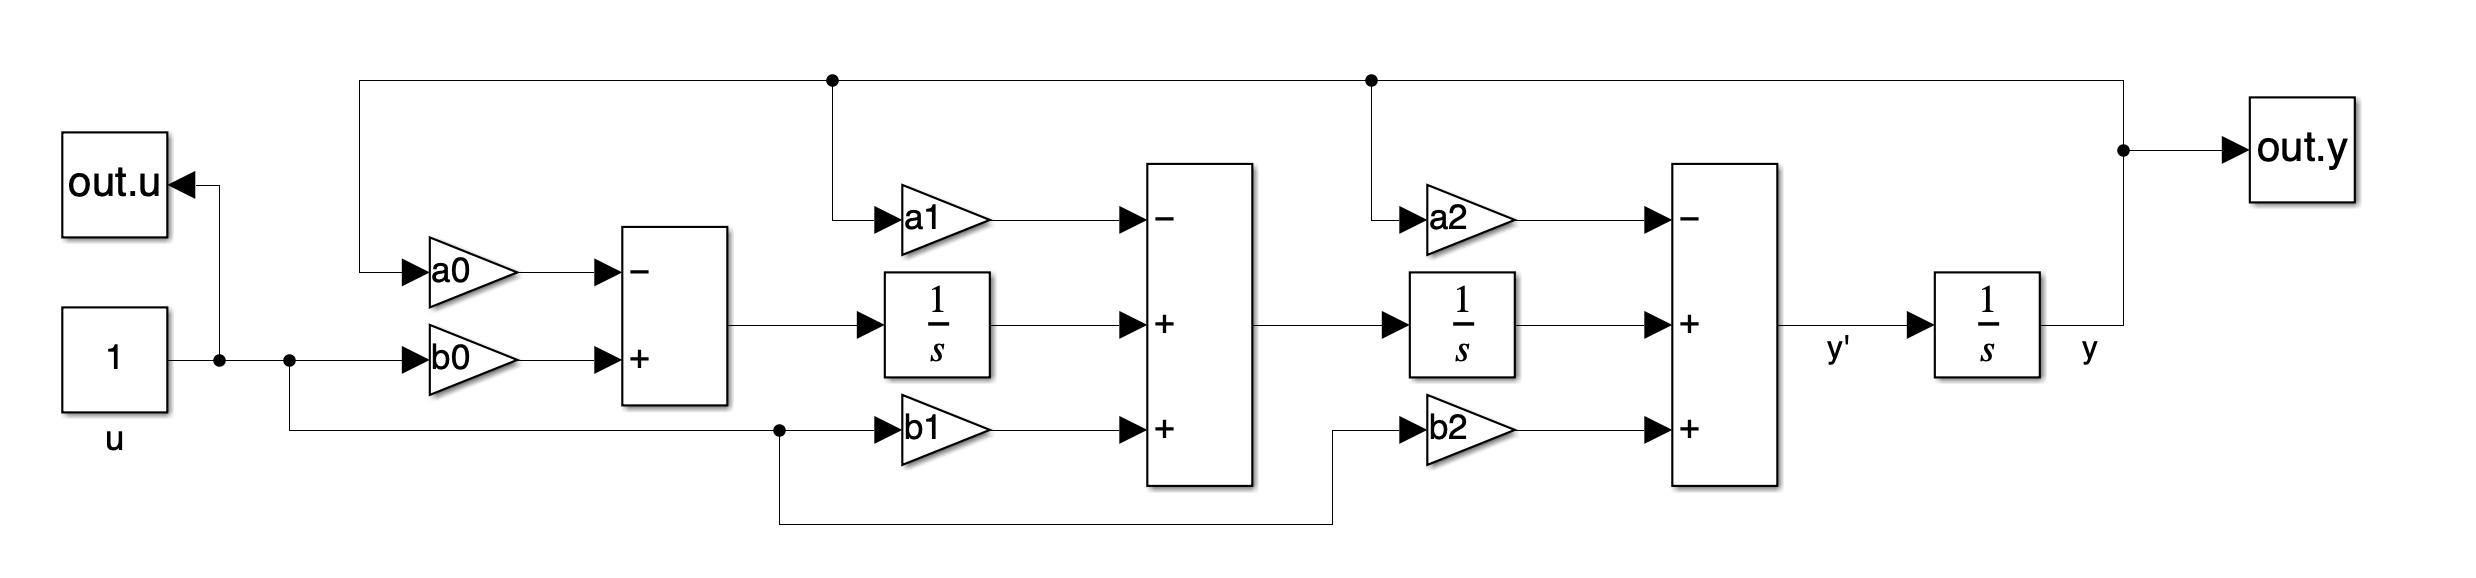
\includegraphics[width=\textwidth]{media/system.png}
    \caption{Схема моделирования одноканальной системы в форме вход-выход}
    \label{fig:model1}
\end{figure}

При этом, начальные условия $\dddot{y}(0) = 0, \ddot{y}(0) = 0, \dot{y}(0) = 0$ задаются в блоках \textit{Integrator}.

Промоделировав данную систему получим графики $y(t)$ и $u(t)$ (рис. \ref{fig:yt}, \ref{fig:ut}).

\begin{figure}
    \centering
    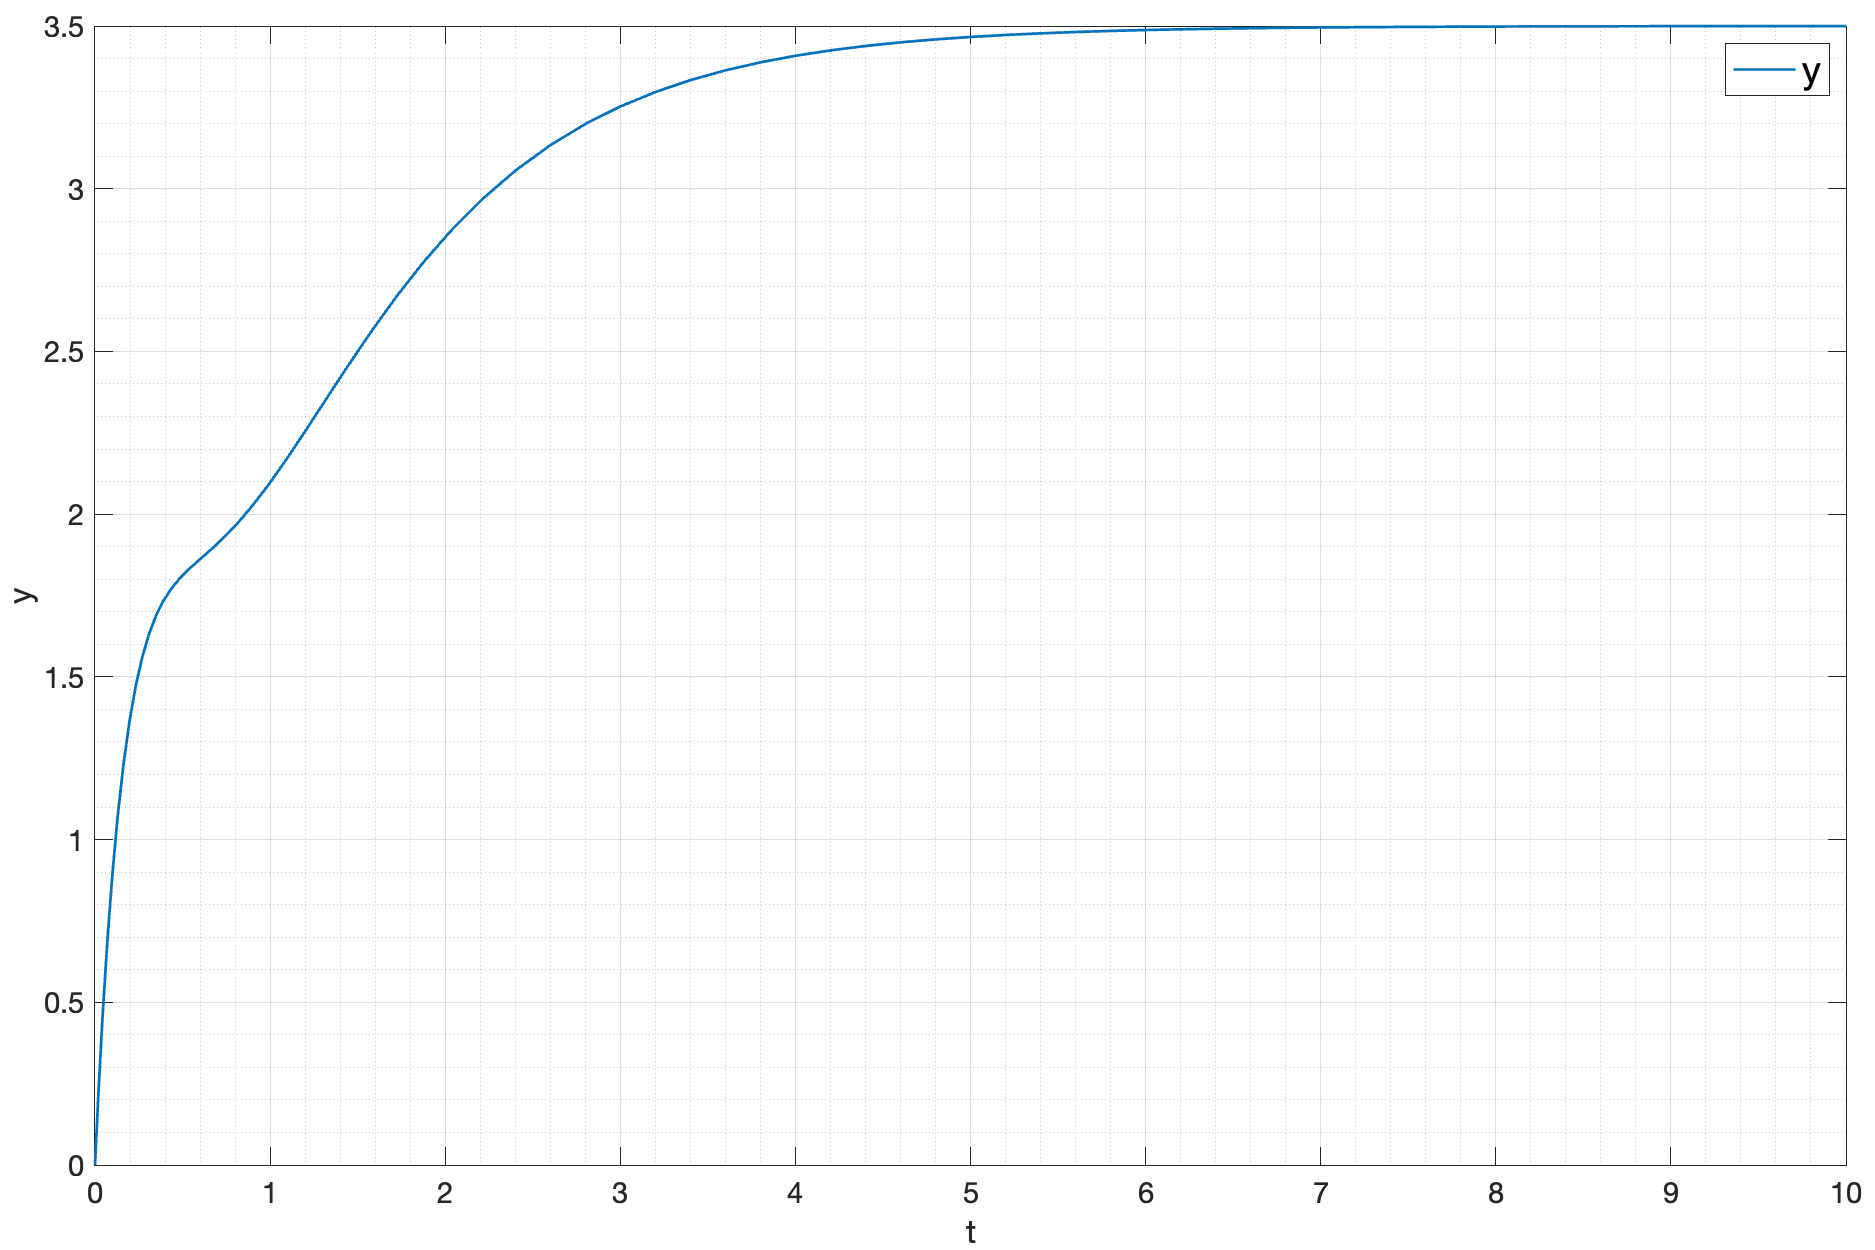
\includegraphics[width=\textwidth]{media/sys1_y(t).png}
    \caption{График $y(t)$}
    \label{fig:yt}
\end{figure}

\begin{figure}
    \centering
    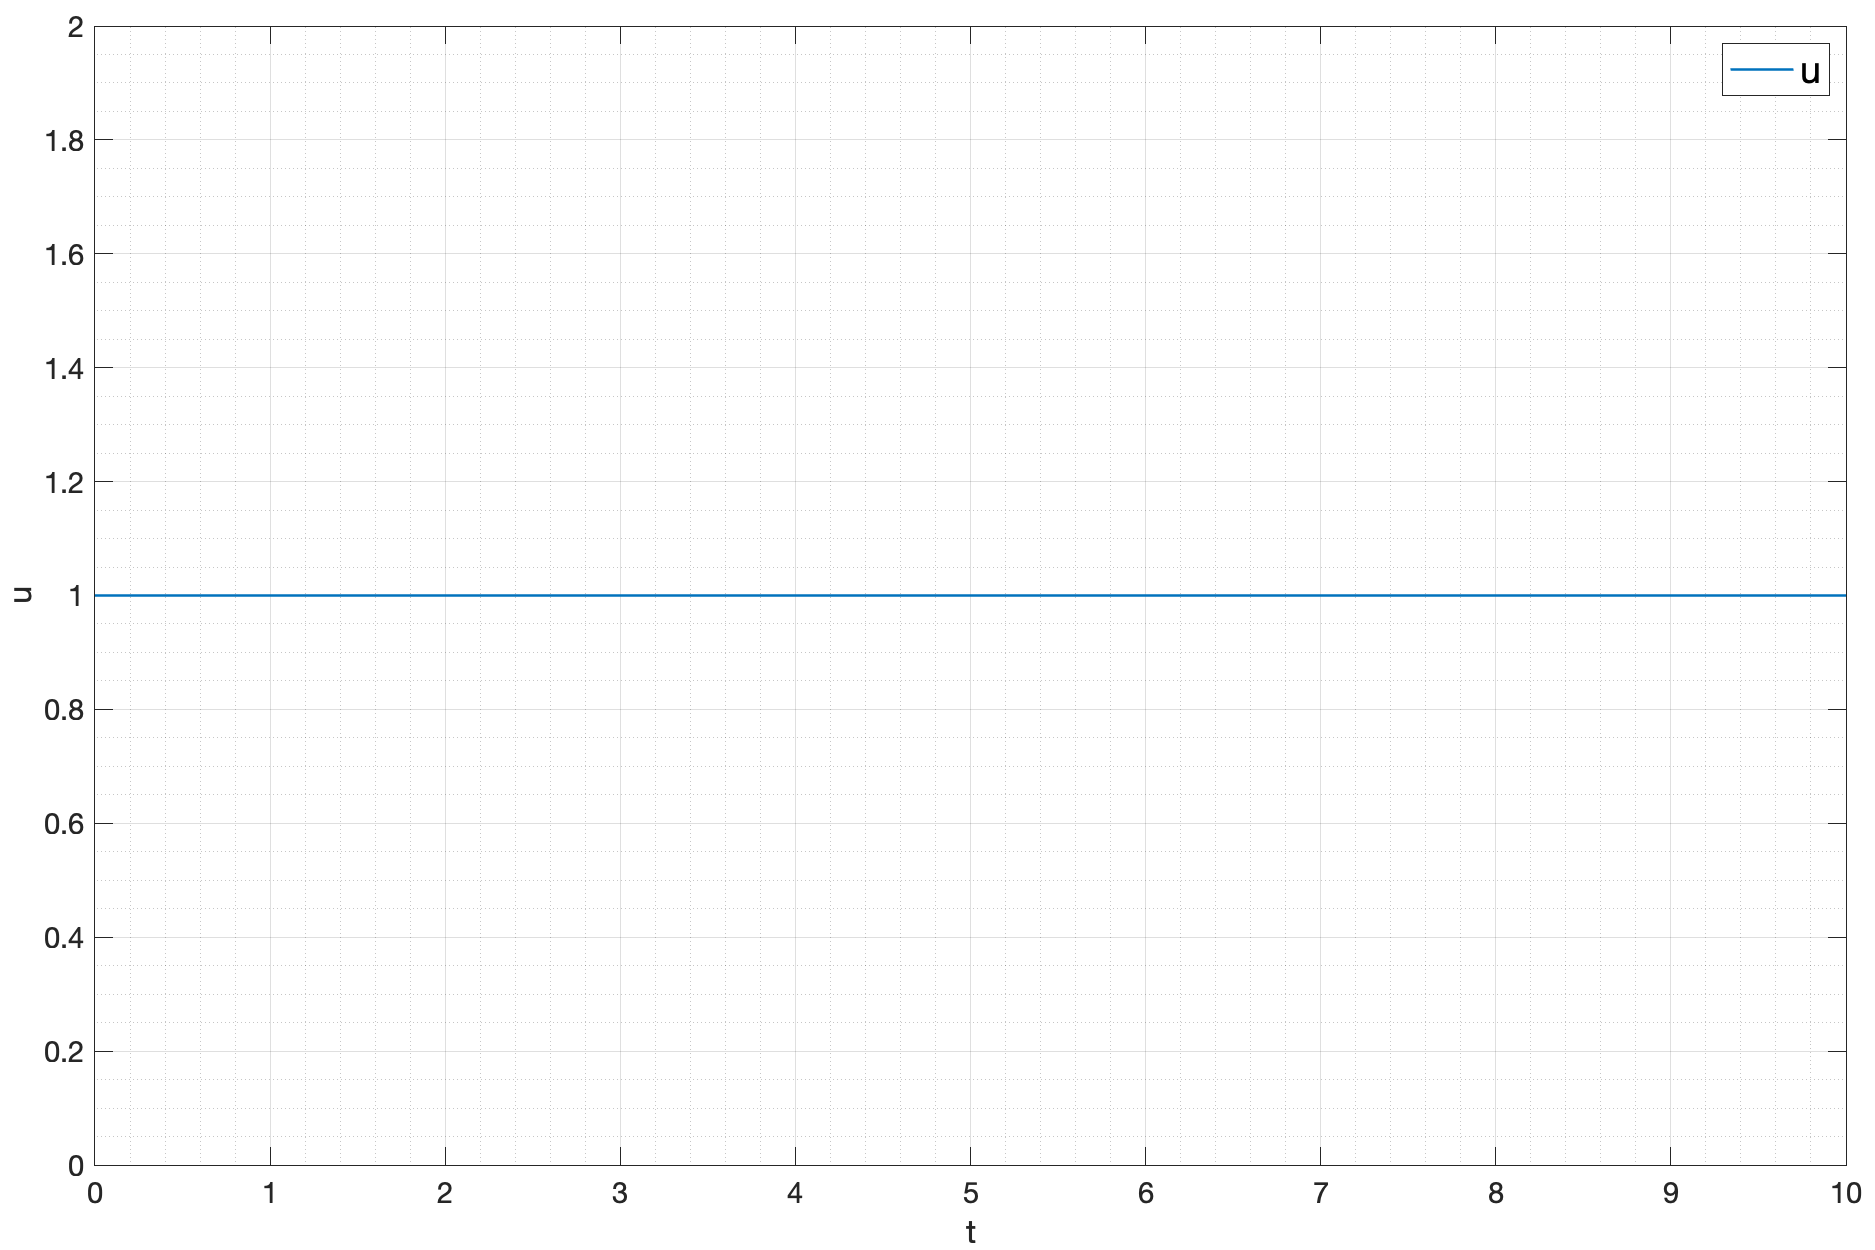
\includegraphics[width=\textwidth]{media/sys1_u(t).png}
    \caption{График $u(t)$}
    \label{fig:ut}
\end{figure}
